\cleardoublepage%
\chapter{\label{chap:res}Results and Discussion}%

%This is where you present your findings. As much as possible, structure your results along the lines of your research questions. Start with the simplest results first and proceed to more complex ones. Tables and Figures should be clear enough that they need little explanation: do not simply re-write the numbers as text to fill space. Rather, highlight trends, outliers, or gaps. 

\section{\label{sec:res_networking}Networking}%should this be in firmware?

In line with research question 1, we present the networking structure, which enables communication and blahbalhbalh

\subsection{\label{sec:res_logic}Concept, Structure and Logic}

As outlined in Section \ref{sec:methods_net_des} and Section \ref{sec:methods_net_dev}, the networking was designed and developed in two parts, the base networking.py library and using the interfaces of the base networking as a base, the more specific ssp\_networking.py. \\

The base networking.py library is designed to be a general purpose library that builds on ESP-NOW and adds some basic structure and functionality. This base networking introduces address book logic that bypasses ESP-NOW's 20 peer limit, allowing transmission to a theoretically unlimited number of peers at the expense of efficiency. It also introduces the basic message structure, including different message types (cmd, inf, ack) and different subtypes (cmd: ping, echo, boop; inf: msg, data; ack: pong, echo, boop). The library also includes logic to send data larger than $241\ bytes$, the maximum payload allowed using the message structure defined in Section \ref{sec:rev_net}, increasing it to a theoretical limit of $60'928\ bytes$. However, in reality the message limit is lower, with the maximum amount successfully transmitted at about 30 kB due to the memory limitations of the MicroPython firmware running on the ESP32C3. Also, sending large messages in chunks runs the risk of some chunks being lost during transmission (see Section \ref{sec:res_rssi}), especially over long distances, resulting in the entire message being dropped. While there is a provision in the code to remedy this by storing all parts of a long message in a buffer, and if the receiving device is missing one or more parts of a multi-part message after some time, it sends a message requesting the missing parts, this has been disabled for memory optimisation. 
The network design also includes various interfaces for customisation and the addition of additional custom commands, message types and handling logic, including custom IRQ messages. \\

Building on top of these interfaces of the base networking library, the SSP networking library introduces many additional smart module specific commands, handlers and message types, which allow the effective control and configuration of smart modules using the appropriate commands.

The specific structure of the code of the two libraries and all its commands is shown in Figure \ref{fig:net_code_structure}
Give a quick overview of the networking structure. 

Overview of networking, recall design requirements and guiding principles.

\begin{figure}[H]
    \centering
    \includegraphics[width=.5\linewidth]{overleaf/images/placeholder.png}
    \vspace{\ftspace}
    \caption{Networking overview}
    \label{fig:Networking overview}
\end{figure}

To ammend this, 
While the structure exists for a recipient to send confirmations, nothing is done with this information so far, though users could decide to build their own handshake logic on top of our networking structure and use this, the necessary ground work is already in place.


In particular, the Networking Library is compatible with the Smart Motors hardware and with any ESP32-based hardware that includes Wi-Fi and thus ESP-NOW capabilities, as well as with the MicroPython firmware used. The protocol uses a peer-to-peer communication approach, inherited from the basic ESP-NOW design on which it is based, and requires no central root or hub or even configuration to use, other than initialising the library. It also includes message validation features, using a common message structure that includes an identifier and checksum, and provisions for easy module discovery, using the ping command defined in the base networking library, and interaction, using the various further defined commands and message types defined in the SSP networking add-on. This further satisfies the latter two. In terms of design principles, the networking is split into two parts, allowing the base networking, which contains simple logic and commands, to be used in a variety of custom ways, and further allowing interfaces for customisation. 

The code is furthermore following the style Guide for Python Code based Python Enhancement Proposal 8. \citep{rossum_python_2001}

\subsection{\label{sec:res_range}Range Test}

As outlined in Section \ref{sec:methods_test_range}, the original range test was conducted using the boop-o-meter program on a street in front of the CEEO offices. The maximum range at which some messages were still being received by each of the two modules was approximately 242 meters, as shown in Figure \ref{sec:res_range}.

\begin{figure}[H]
    \centering
    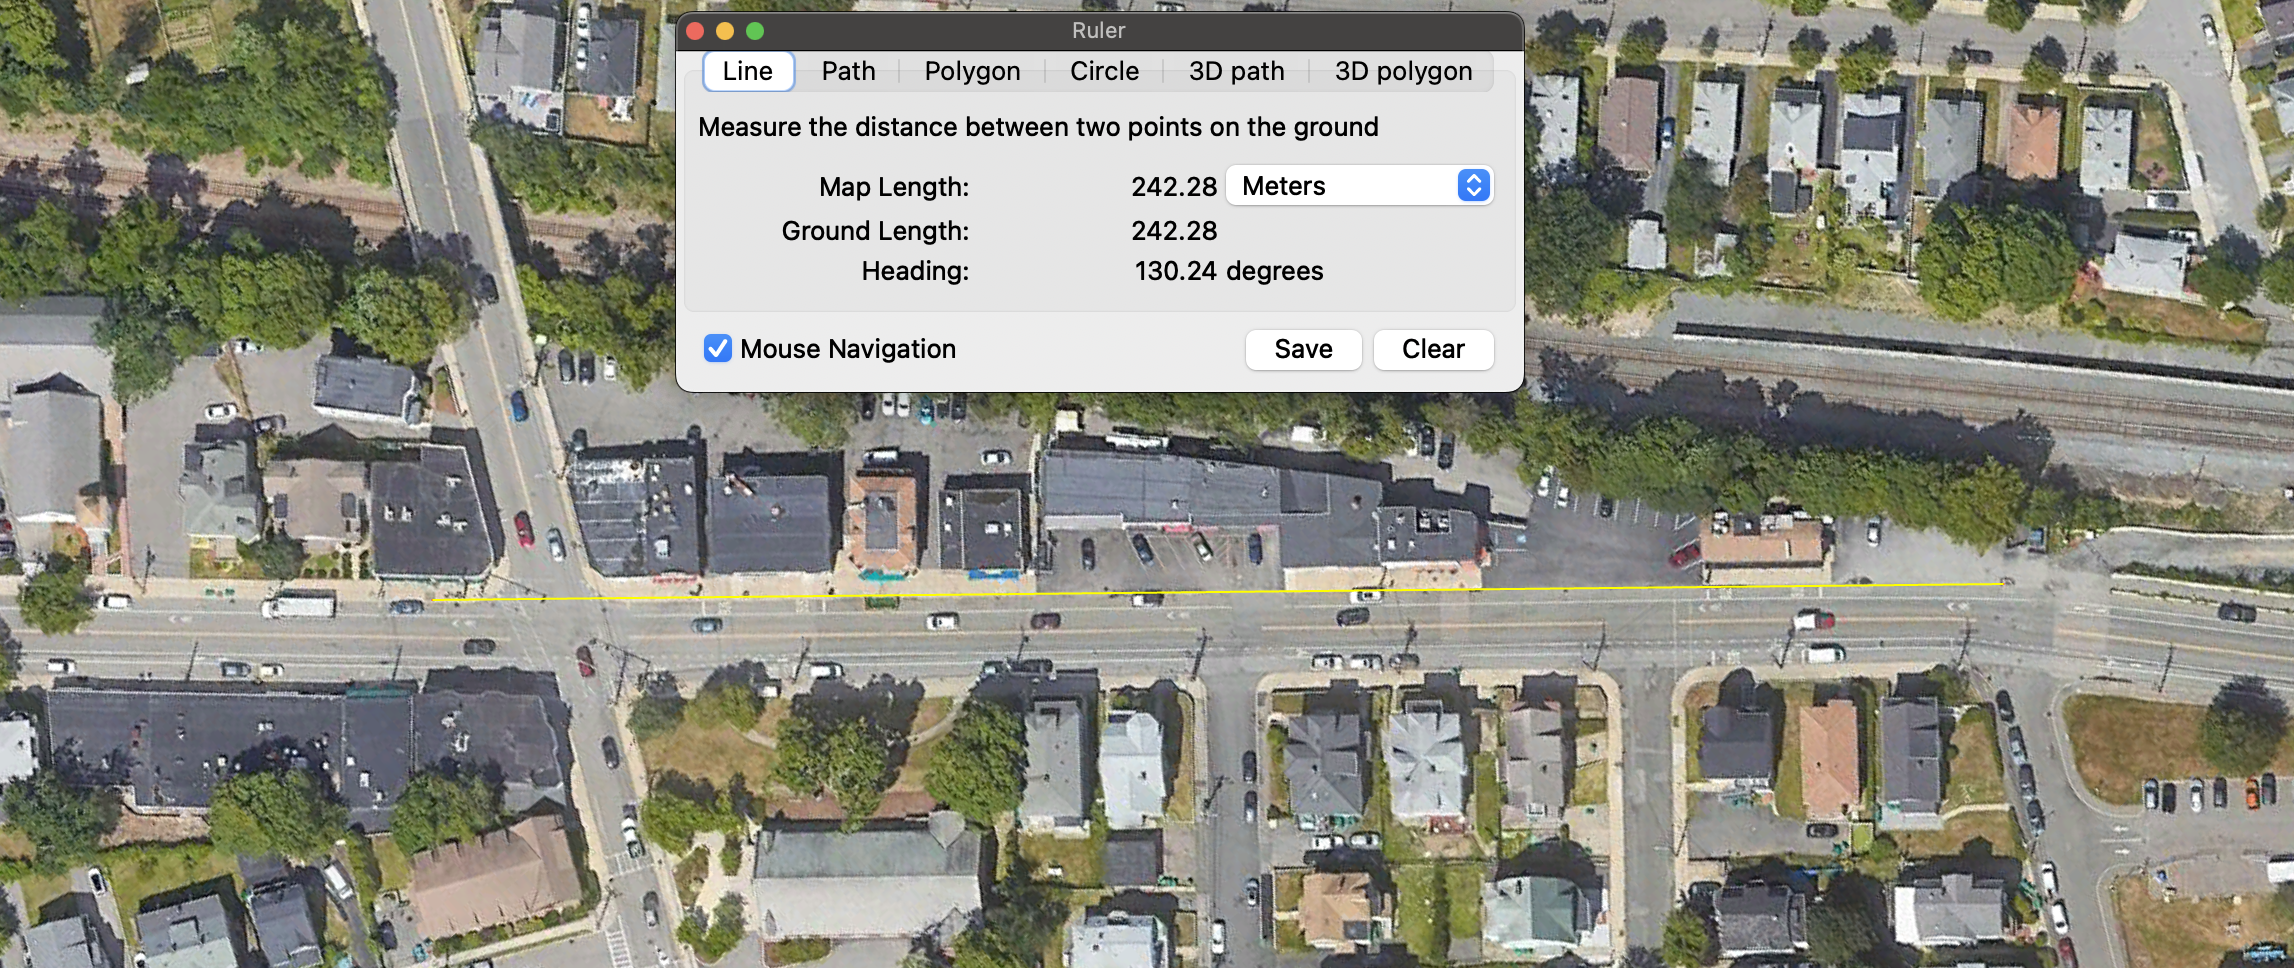
\includegraphics[width=\linewidth]{overleaf/images/range.png}
    \vspace{\ftspace}
    \caption{Approximate Range Test on Boston Avenue, MA}
    \label{fig:range}
\end{figure}


\subsection{\label{sec:res_rssi}Response Time, RSSI and Packet Loss Rate by Range}

The RSSI, ping response and packege loss for various ranges was measured three times using two ESP32C3s, one ESP32C3 and one ESP32C6 and again using two ESP32C6s.

\subsubsection{ESP32C3 to ESP32C3}

\begin{figure}[H]
    \centering
    \begin{subfigure}{0.45\textwidth}
        \includegraphics[width=\linewidth]{rstudio/analysis/plots/ESP32C3_rssi_box.png}
    \end{subfigure}
    \begin{subfigure}{0.45\textwidth}
        \includegraphics[width=\linewidth]{rstudio/analysis/plots/ESP32C3_avg_rssi.png}
    \end{subfigure}

    \begin{subfigure}{0.45\textwidth}
        \includegraphics[width=\linewidth]{rstudio/analysis/plots/ESP32C3_ping_box.png}
    \end{subfigure}
    \begin{subfigure}{0.45\textwidth}
        \includegraphics[width=\linewidth]{rstudio/analysis/plots/ESP32C3_avg_ping.png}
    \end{subfigure}
    \vspace{\ftspace}
    \caption{RSSI and Ping Time depending on antenna angle}
    \label{fig:rssipingrange_esp32c3}
\end{figure}

As expected, the RSSI values, an index for signal strength, drops for longer ranges, following a logarithmic curve, as shown in Figure \ref{sec:res_rssi}. The RSSI values for both devices are very similar and also follow a similar curve, with a slight divergence, which could be explained by differences in production quality of the antenna. Together with the increase of negative values, 

In terms of ping time, the averages are not affected by range, which makes sense as the increase in travel time from 0 to 100 meters is only approximately $0.0000033356\ ms$ ($100\ m\ /\ 299'792'000'000\ m/ms$), which is insignificant compared to the time taken by the MCB to process it. Interestingly, the values tend to cluster at specific values with a distance of $10\ ms$, either $10\ ms$, $20\ ms$ or $30\ ms$, which might be caused by an underlying system clock rate of the MCB. There are various outliers in terms of ping time, more notably for the larger distances, though also for the measurements at 1 and 0.5 meters. The outliers of these two measurements were the first measurements of the tests, both likely taken after a restart of the used ESP32 MCBs. As such, the code had to add the peer it received the message from to its ESP-NOW buffer, which might explain some of the delay and the high ping response time for the first measurement. Subsequent measurements taken at the same distance, for example for the angle tests in Section \ref{sec:res_angle}, did not yield any such outliers, however most measurements after restart of the device, did. For other test sessions the code was usually tested in a first trial run, whose data was disregarded, which might be why this is only apparent for these two specific measurements.

As for packet loss, transmission remains lossless until 25 meters, at which point packets start to become lost. These values increase with distance, with about one third of packages lost at a distance of 100 meters, as shown in Table \ref{tab:rssipingrange_esp32c3}.

\begin{table}[H]
    \centering
    \begin{tabular}{|c|c|l|l|c|c|c|c|c|}
    \hline
        Range & Packet Loss & \multicolumn{2}{l|}{Measurement} & \multicolumn{5}{c|}{Values} \\\hline
        [meters] & [\%] & \multicolumn{2}{l|}{} & mean & std & min & max & median \\\hline\hline
        \multirow{3}{*}{0 m} & \multirow{1}{*}{0} & RSSI 1 & [asu] & -6.05 & 1.14 & -12 & -5 & -6 \\\cline{2-9}\cline{2-9}
        %&& Time 1 &  &  &  &  &  \\\cline{2-9}\cline{2-9}
        & \multirow{2}{*}{0} & RSSI 2 & [asu] & -5.44 & 0.67 & -8 & -5 & -5 \\\cline{3-9}
        %&& Time 2 &  &  &  &  &  \\\cline{3-9}
        && Ping & [ms] & 20.57 & 0.61 & 19 & 23 & 20 \\\hline\hline
        \multirow{3}{*}{0.1 m} & \multirow{1}{*}{0} & RSSI 1 & [asu] & -15.5 & 0.59 & -17 & -15 & -15 \\\cline{2-9}\cline{2-9}
        %&& Time 1 &  &  &  &  &  \\\cline{2-9}\cline{2-9}
        & \multirow{2}{*}{0} & RSSI 2 & [asu] & -15.25 & 0.54 & -16 & -14 & -15 \\\cline{3-9}
        %&& Time 2 &  &  &  &  &  \\\cline{3-9}
        && Ping & [ms] & 20.36 & 1.08 & 19 & 30 & 20 \\\hline\hline
        \multirow{3}{*}{0.25 m} & \multirow{1}{*}{0} & RSSI 1 & [asu] & -20.59 & 0.72 & -23 & -20 & -20 \\\cline{2-9}\cline{2-9}
        %&& Time 1 &  &  &  &  &  \\\\cline{2-9}\cline{2-9}
        & \multirow{2}{*}{0} & RSSI 2 & [asu] & -20.58 & 0.53 & -22 & -20 & -21 \\\cline{3-9}
        %&& Time 2 &  &  &  &  &  \\\cline{3-9}
        && Ping & [ms] & 20.16 & 0.58 & 17 & 21 & 20 \\\hline\hline
        \multirow{3}{*}{0.5 m} & \multirow{1}{*}{0} & RSSI 1 & [asu] & -27.22 & 0.73 & -29 & -25 & -27 \\\cline{2-9}\cline{2-9}
        %&& Time 1 &  &  &  &  &  \\\cline{2-9}\cline{2-9}
        & \multirow{2}{*}{0} & RSSI 2 & [asu] & -27.15 & 0.77 & -30 & -25 & -27 \\\cline{3-9}
        %&& Time 2 &  &  &  &  &  \\\cline{3-9}
        && Ping & [ms] & 23.32 & 22.42 & 19 & 223 & 20 \\\hline\hline
        \multirow{3}{*}{1 m} & \multirow{1}{*}{0} & RSSI 1 & [asu] & -31.14 & 0.93 & -33 & -29 & -31 \\\cline{2-9}\cline{2-9}
        %&& Time 1 &  &  &  &  &  \\\cline{2-9}\cline{2-9}
        & \multirow{2}{*}{0} & RSSI 2 & [asu] & -31.18 & 0.74 & -29 & -33 & -31 \\\cline{3-9}
        %&& Time 2 &  &  &  &  &  \\\cline{3-9}
        && Ping & [ms] & 23.29 & 22.11 & 19 & 219 & 20 \\\hline\hline
        \multirow{3}{*}{5 m} & \multirow{1}{*}{0} & RSSI 1 & [asu] & -42.67 & 0.97 & -45 & -41 & -43 \\\cline{2-9}\cline{2-9}
        %&& Time 1 &  &  &  &  &  \\\cline{2-9}\cline{2-9}
        & \multirow{2}{*}{0} & RSSI 2 & [asu] & -44.91 & 2.87 & -72 & -42 & -45 \\\cline{3-9}
        %&& Time 2 &  &  &  &  &  \\\cline{3-9}
        && Ping & [ms] & 22.47 & 9.34 & 10 & 50 & 20 \\\hline\hline
        \multirow{3}{*}{10 m} & \multirow{1}{*}{0} & RSSI 1 & [asu] & -45.03 & 1.23 & -50 & -43 & -45 \\\cline{2-9}\cline{2-9}
        %&& Time 1 &  &  &  &  &  \\\cline{2-9}\cline{2-9}
        & \multirow{2}{*}{0} & RSSI 2 & [asu] & -46.83 & 1.01 & -50 & -45 & -47 \\\cline{3-9}
        %&& Time 2 &  &  &  &  &  \\\cline{3-9}
        && Ping & [ms] & 19.8 & 7.52 & 10 & 41 & 20 \\\hline\hline
        \multirow{3}{*}{25 m} & \multirow{1}{*}{3} & RSSI 1 & [asu] & -62.54 & 3.17 & -87 & -57 & -63 \\\cline{2-9}\cline{2-9}
        %&& Time 1 &  &  &  &  &  \\\cline{2-9}\cline{2-9}
        & \multirow{2}{*}{3} & RSSI 2 & [asu] & -64.72 & 2.04 & -71 & -60 & -65 \\\cline{3-9}
        %&& Time 2 &  &  &  &  &  \\\cline{3-9}
        && Ping & [ms] & 18.88 & 7.46 & 9 & 41 & 20 \\\hline\hline
        \multirow{3}{*}{50 m} & \multirow{1}{*}{12} & RSSI 1 & [asu] & -65.69 & 2.38 & -73 & -62 & -65 \\\cline{2-9}\cline{2-9}
        %&& Time 1 &  &  &  &  &  \\\\cline{2-9}\cline{2-9}
        & \multirow{2}{*}{12} & RSSI 2 & [asu] & -68.08 & 2.38 & -74 & -64 & -68 \\\cline{3-9}
        %&& Time 2 &  &  &  &  &  \\\cline{3-9}
        && Ping & [ms] & 20.95 & 11.22 & 10 & 91 & 20 \\\hline\hline
        \multirow{3}{*}{100 m} & \multirow{1}{*}{32} & RSSI 1 & [asu] & -70.12 & 3.61 & -82 & -63 & -69 \\\cline{2-9}\cline{2-9}
        %&& Time 1 &  &  &  &  &  \\\cline{2-9}\cline{2-9}
        & \multirow{2}{*}{34} & RSSI 2 & [asu] & -73.52 & 3.27 & -86 & -66 & -73 \\\cline{3-9}
        %&& Time 2 &  &  &  &  &  \\\cline{3-9}
        && Ping & [ms] & 26.29 & 18.17 & 10 & 141 & 20 \\\hline
    \end{tabular}
    \vspace{\ftspace}
    \caption{RSSI, ping time and package loss measurements for various ranges}
    \label{tab:rssipingrange_esp32c3}
\end{table}

\subsubsection{ESP32C3 to ESP32C6}

\begin{figure}[H]
    \centering
    \begin{subfigure}{0.45\textwidth}
        \includegraphics[width=\linewidth]{rstudio/analysis/plots/ESP32C36_rssi_box.png}
    \end{subfigure}
    \begin{subfigure}{0.45\textwidth}
        \includegraphics[width=\linewidth]{rstudio/analysis/plots/ESP32C36_avg_rssi.png}
    \end{subfigure}

    \begin{subfigure}{0.45\textwidth}
        \includegraphics[width=\linewidth]{rstudio/analysis/plots/ESP32C36_ping_box.png}
    \end{subfigure}
    \begin{subfigure}{0.45\textwidth}
        \includegraphics[width=\linewidth]{rstudio/analysis/plots/ESP32C36_avg_ping.png}
    \end{subfigure}
    \vspace{\ftspace}
    \caption{RSSI and Ping response time depending on range}
    \label{fig:rssipingrange_esp32c36}
\end{figure}

Similar results were obtained using an ESP32C3 as the sender and an ESP32C6 as the receiver, the RSSI values followed a similar logarithmic path, although in this case the values were much lower for both devices, probably due to the lower on-board antenna used by the ESP32C6. The RSSI values for the sender (ESP32C3) remained significantly higher for most measurements, except for the 5 meter and 50 meter measurements where the values were similar. Surprisingly, the RSSI values for 100 meters were better than both 50 and 25 meters, with the lowest values for the test occurring at 25 meters. Ping values were also similar across the board, averaging around $20\ ms$, with some small outliers at longer distances.5
In terms of packet loss, the trend seen for RSSI values is repeated, packet loss is highest for the measurement of 25 meters, with a similar amount of packets lost per way. Surprisingly, no packets were lost for the measurement at 100 meters. 
There also seems to be an unexplained inconsistency in the data, specifically for the 10 meter measurement, the echo device did not receive two packets (number 62 and 72), but the sender did receive the return echo of these two packets. Something is obviously wrong here, but in the raw data collected, packets 62 and 72 are marked as received with a timestamp for the sender, whereas there are no entries for number 62 and 72 for the echo device. It has been considered whether an inaccuracy in the test code could have caused this, for example the dictionary not being cleared or reinitialised with previous values stored, but this seems improbable, as a dictionary is cleared and reinitialised as empty with every new run of the code as well as when data is written to files. although this seems unlikely as the timestamps match the surrounding entries. There could also have been an error on the part of the echoer in writing the data to the dictionary. As the response and echo logic is based on IRQ functions, an error would not have interrupted the code, so this may have gone unnoticed, but there seems no satisfactory way of explaining this inconsistency in the data. 

\begin{table}[H]
    \centering
    \begin{tabular}{|c|c|l|l|c|c|c|c|c|}
    \hline
        Range & Packet Loss & \multicolumn{2}{l|}{Measurement} & \multicolumn{5}{c|}{Values} \\\hline
        [meters] & [\%] & \multicolumn{2}{l|}{} & mean & std & min & max & median \\\hline\hline
        \multirow{3}{*}{0 m} & \multirow{1}{*}{0} & RSSI 1 & [asu] & -6.05 & 1.14 & -12 & -5 & -6 \\\cline{2-9}\cline{2-9}
        %&& Time 1 &  &  &  &  &  \\\cline{2-9}\cline{2-9}
        & \multirow{2}{*}{0} & RSSI 2 & [asu] & -27.13 & 0.93 & -29 & -26 & -27 \\\cline{3-9}
        %&& Time 2 &  &  &  &  &  \\\cline{3-9}
        && Ping & [ms] & 20.98 & 0.14 & 20 & 21 & 21 \\\hline\hline
        \multirow{3}{*}{0.1 m} & \multirow{1}{*}{0} & RSSI 1 & [asu] & -46.43 & 1.12 & -44 & -48 & -46 \\\cline{2-9}\cline{2-9}
        %&& Time 1 &  &  &  &  &  \\\cline{2-9}\cline{2-9}
        & \multirow{2}{*}{0} & RSSI 2 & [asu] & -38.22 & 1.04 & -41 & -36 & -38 \\\cline{3-9}
        %&& Time 2 &  &  &  &  &  \\\cline{3-9}
        && Ping & [ms] & 20.96 & 0.24 & 19 & 21 & 21 \\\hline\hline
        \multirow{3}{*}{0.25 m} & \multirow{1}{*}{0} & RSSI 1 & [asu] & -52.86 & 0.72 & -54 & -51 & -53 \\\cline{2-9}\cline{2-9}
        %&& Time 1 &  &  &  &  &  \\\\cline{2-9}\cline{2-9}
        & \multirow{2}{*}{0} & RSSI 2 & [asu] & -41.97 & 1.02 & -47 & -40 & -42 \\\cline{3-9}
        %&& Time 2 &  &  &  &  &  \\\cline{3-9}
        && Ping & [ms] & 20.97 & 0.17 & 20 & 21 & 21 \\\hline\hline
        \multirow{3}{*}{0.5 m} & \multirow{1}{*}{0} & RSSI 1 & [asu] & -50.61 & 0.72 & -52 & -48 & -51 \\\cline{2-9}\cline{2-9}
        %&& Time 1 &  &  &  &  &  \\\cline{2-9}\cline{2-9}
        & \multirow{2}{*}{0} & RSSI 2 & [asu] & -39.26 & 0.66 & -42 & -38 & -39 \\\cline{3-9}
        %&& Time 2 &  &  &  &  &  \\\cline{3-9}
        && Ping & [ms] & 20.92 & 0.52 & 16 & 21 & 21 \\\hline\hline
        \multirow{3}{*}{1 m} & \multirow{1}{*}{0} & RSSI 1 & [asu] & -60.58 & 1.39 & -68 & -59 & -60.5 \\\cline{2-9}\cline{2-9}
        %&& Time 1 &  &  &  &  &  \\\cline{2-9}\cline{2-9}
        & \multirow{2}{*}{0} & RSSI 2 & [asu] & -53.84 & 1.6 & -63 & -50 & -53 \\\cline{3-9}
        %&& Time 2 &  &  &  &  &  \\\cline{3-9}
        && Ping & [ms] & 20.95 & 0.33 & 18 & 21 & 21 \\\hline\hline
        \multirow{3}{*}{5 m} & \multirow{1}{*}{0} & RSSI 1 & [asu] & -74.77 & 0.42 & -75 & -74 & -75 \\\cline{2-9}\cline{2-9}
        %&& Time 1 &  &  &  &  &  \\\cline{2-9}\cline{2-9}
        & \multirow{2}{*}{0} & RSSI 2 & [asu] & -74.36 & 0.76 & -76 & -72 & -74 \\\cline{3-9}
        %&& Time 2 &  &  &  &  &  \\\cline{3-9}
        && Ping & [ms] & 20.9 & 0.81 & 13 & 21 & 21 \\\hline\hline
        \multirow{3}{*}{10 m} & \multirow{1}{*}{2} & RSSI 1 & [asu] & -88.48 & 2.02 & -93 & -83 & -89 \\\cline{2-9}\cline{2-9}
        %&& Time 1 &  &  &  &  &  \\\cline{2-9}\cline{2-9}
        & \multirow{2}{*}{0} & RSSI 2 & [asu] & -77.89 & 0.87 & -82 & -75 & -78 \\\cline{3-9}
        %&& Time 2 &  &  &  &  &  \\\cline{3-9}
        && Ping & [ms] & 20.94 & 0.42 & 17 & 21 & 21 \\\hline\hline
        \multirow{3}{*}{25 m} & \multirow{1}{*}{17} & RSSI 1 & [asu] & -93.24 & 2.51 & -98 & -88 & -94 \\\cline{2-9}\cline{2-9}
        %&& Time 1 &  &  &  &  &  \\\cline{2-9}\cline{2-9}
        & \multirow{2}{*}{26} & RSSI 2 & [asu] & -90.73 & 1.33 & -95 & -86 & -91 \\\cline{3-9}
        %&& Time 2 &  &  &  &  &  \\\cline{3-9}
        && Ping & [ms] & 22.78 & 4.31 & 16 & 41 & 21 \\\hline\hline
        \multirow{3}{*}{50 m} & \multirow{1}{*}{0} & RSSI 1 & [asu] & -88.18 & 1.49 & -94 & -86 & -88 \\\cline{2-9}\cline{2-9}
        %&& Time 1 &  &  &  &  &  \\\\cline{2-9}\cline{2-9}
        & \multirow{2}{*}{6} & RSSI 2 & [asu] & -89.67 & 1.73 & -95 & -84 & -90 \\\cline{3-9}
        %&& Time 2 &  &  &  &  &  \\\cline{3-9}
        && Ping & [ms] & 23.74 & 4.94 & 20 & 41 & 21 \\\hline\hline
        \multirow{3}{*}{100 m} & \multirow{1}{*}{0} & RSSI 1 & [asu] & -86.9 & 1.17 & -89 & -84 & -87 \\\cline{2-9}\cline{2-9}
        %&& Time 1 &  &  &  &  &  \\\cline{2-9}\cline{2-9}
        & \multirow{2}{*}{0} & RSSI 2 & [asu] & -78.95 & 1.6 & -83 & -75 & -79 \\\cline{3-9}
        %&& Time 2 &  &  &  &  &  \\\cline{3-9}
        && Ping & [ms] & 21.25 & 1.76 & 17 & 31 & 21 \\\hline
    \end{tabular}
    \vspace{\ftspace}
    \caption{RSSI, ping time and package loss measurements for various ranges}
    \label{tab:rssipingrange_esp32c36}
\end{table}

\subsubsection{ESP32C6 to ESP32C6}

\begin{figure}[H]
    \centering
    \begin{subfigure}{0.45\textwidth}
        \includegraphics[width=\linewidth]{rstudio/analysis/plots/ESP32C6_rssi_box.png}
    \end{subfigure}
    \begin{subfigure}{0.45\textwidth}
        \includegraphics[width=\linewidth]{rstudio/analysis/plots/ESP32C6_avg_rssi.png}
    \end{subfigure}

    \begin{subfigure}{0.45\textwidth}
        \includegraphics[width=\linewidth]{rstudio/analysis/plots/ESP32C6_ping_box.png}
    \end{subfigure}
    \begin{subfigure}{0.45\textwidth}
        \includegraphics[width=\linewidth]{rstudio/analysis/plots/ESP32C6_avg_ping.png}
    \end{subfigure}
    \vspace{\ftspace}
    \caption{RSSI and Ping Time depending on antenna angle using two ESP32C6s}
    \label{fig:rssipingrange_esp32c6}
\end{figure}

However, when using two ESP32C6s, there were problems with transmission over a distance of more than 15 meters. As transmission with an ESP32C3 (sender) and an ESP32C6 (echo) was achieved up to 100 meters, the experiment was repeated with the ESP32C6 chip as the sender, which hadn't been validated in a previous test, but each time with different chips there were similar results, although in some trials the maximum distance was even lower. One suspicion for the cause of these problems was problems with the antenna, or rather the wrong antenna being used. As the MCB has two antennas, a built-in one and a connector, it is suspected that it may have been using the antenna connector (which allows short range transmission even when no antenna is connected). However, the chips are set to use the on-board antenna by default, and they seem to be set correctly. Another suspicion is hardware problems, but the ESP32C3 was able to transmit over longer distances using the same ESP32C6 chips that were used in a test with each other. Another possibility is that the problem is caused by the smaller on-board antenna of the ESP32C6. 
In terms of RSSI values, the overall values were lower compared to the test with an ESP32C3 and an ESP32C6, which could also be explained by the two smaller antennas. The results also follow an expected logarithmic curve for the last measurement at 15 meters, where the RSSI values of the receiver are much higher compared to the immediately lower ranges and also compared to the RSSI values of the sender. However, this data-point is only compromised by four values due to the very high packet loss at 15 meters.
As for the ping values, they are consistent as expected, although they are slightly lower at higher ranges.
Locking at packet loss, minimal packages were lost for 5 and 10 meters respectively, however, at 15 meters 95 packets were lost on the return transmission.

\begin{table}[H]
    \centering
    \begin{tabular}{|c|c|l|l|c|c|c|c|c|}
    \hline
        Range & Packet Loss & \multicolumn{2}{l|}{Measurement} & \multicolumn{5}{c|}{Values} \\\hline
        [meters] & [\%] & \multicolumn{2}{l|}{} & mean & std & min & max & median \\\hline\hline
        \multirow{3}{*}{0 m} & \multirow{1}{*}{0} & RSSI 1 & [asu] & -38.27 & 1.98 & -42 & -37 & -37 \\\cline{2-9}\cline{2-9}
        %&& Time 1 &  &  &  &  &  \\\cline{2-9}\cline{2-9}
        & \multirow{2}{*}{0} & RSSI 2 & [asu] & -38.14 & 1.97 & -42 & -36 & -37 \\\cline{3-9}
        %&& Time 2 &  &  &  &  &  \\\cline{3-9}
        && Ping & [ms] & 19.93 & 0.55 & 15 & 21 & 20 \\\hline\hline
        \multirow{3}{*}{0.1 m} & \multirow{1}{*}{0} & RSSI 1 & [asu] & -65.51 & 0.74 & -68 & -65 & -65 \\\cline{2-9}\cline{2-9}
        %&& Time 1 &  &  &  &  &  \\\cline{2-9}\cline{2-9}
        & \multirow{2}{*}{0} & RSSI 2 & [asu] & -65.23 & 0.66 & -67 & -64 & -65 \\\cline{3-9}
        %&& Time 2 &  &  &  &  &  \\\cline{3-9}
        && Ping & [ms] & 19.92 & 0.9 & 11 & 21 & 20 \\\hline\hline
        \multirow{3}{*}{0.25 m} & \multirow{1}{*}{0} & RSSI 1 & [asu] & -74.88 & 0.64 & -76 & -70 & -75 \\\cline{2-9}\cline{2-9}
        %&& Time 1 &  &  &  &  &  \\\\cline{2-9}\cline{2-9}
        & \multirow{2}{*}{0} & RSSI 2 & [asu] & -74.64 & 0.54 & -76 & -73 & -75 \\\cline{3-9}
        %&& Time 2 &  &  &  &  &  \\\cline{3-9}
        && Ping & [ms] & 20 & 0.14 & 19 & 21 & 20 \\\hline\hline
        \multirow{3}{*}{0.5 m} & \multirow{1}{*}{0} & RSSI 1 & [asu] & -75.16 & 0.61 & -77 & -73 & -75 \\\cline{2-9}\cline{2-9}
        %&& Time 1 &  &  &  &  &  \\\cline{2-9}\cline{2-9}
        & \multirow{2}{*}{0} & RSSI 2 & [asu] & -74.66 & 0.53 & -76 & -73 & -75 \\\cline{3-9}
        %&& Time 2 &  &  &  &  &  \\\cline{3-9}
        && Ping & [ms] & 19.94 & 0.53 & 15 & 21 & 20 \\\hline\hline
        \multirow{3}{*}{1 m} & \multirow{1}{*}{2} & RSSI 1 & [asu] & -86.83 & 2.98 & -93 & -80 & -88 \\\cline{2-9}\cline{2-9}
        %&& Time 1 &  &  &  &  &  \\\cline{2-9}\cline{2-9}
        & \multirow{2}{*}{2} & RSSI 2 & [asu] & -86.31 & 2.82 & -92 & -79 & -87 \\\cline{3-9}
        %&& Time 2 &  &  &  &  &  \\\cline{3-9}
        && Ping & [ms] & 20.06 & 0.42 & 20 & 24 & 20 \\\hline\hline
        \multirow{3}{*}{5 m} & \multirow{1}{*}{1} & RSSI 1 & [asu] & -92.95 & 1.11 & -96 & -90 & -93 \\\cline{2-9}\cline{2-9}
        %&& Time 1 &  &  &  &  &  \\\cline{2-9}\cline{2-9}
        & \multirow{2}{*}{1} & RSSI 2 & [asu] & -91.81 & 1.04 & -95 & -90 & -92 \\\cline{3-9}
        %&& Time 2 &  &  &  &  &  \\\cline{3-9}
        && Ping & [ms] & 10.1 & 1.01 & 9 & 20 & 10 \\\hline\hline
        \multirow{3}{*}{10 m} & \multirow{1}{*}{0} & RSSI 1 & [asu] & -94.73 & 1.3 & -98 & -91 & -95 \\\cline{2-9}\cline{2-9}
        %&& Time 1 &  &  &  &  &  \\\cline{2-9}\cline{2-9}
        & \multirow{2}{*}{3} & RSSI 2 & [asu] & -91 & 1.31 & -91 & -97 & -94 \\\cline{3-9}
        %&& Time 2 &  &  &  &  &  \\\cline{3-9}
        && Ping & [ms] & 10 & 0.14 & 9 & 11 & 10 \\\hline\hline
        \multirow{3}{*}{15 m} & \multirow{1}{*}{1} & RSSI 1 & [asu] & -73.42 & 4.9 & -88 & -66 & -72 \\\cline{2-9}\cline{2-9}
        %&& Time 1 &  &  &  &  &  \\\cline{2-9}\cline{2-9}
        & \multirow{2}{*}{96} & RSSI 2 & [asu] & -93.75 & 0.43 & -94 & -93 & -94 \\\cline{3-9}
        %&& Time 2 &  &  &  &  &  \\\cline{3-9}
        && Ping & [ms] & 10 & 0 & 10 & 10 & 10 \\\hline
    \end{tabular}
    \vspace{\ftspace}
    \caption{RSSI, ping time and package loss measurements for various ranges}
    \label{tab:rssipingrange_esp32c6}
\end{table}

\subsection{\label{sec:res_ping}Networking Library Ping Response Time}

\begin{figure}[H]
    \centering
    \includegraphics[width=.45\textwidth]{rstudio/analysis/plots/ping_net_ping.png}
    \vspace{\ftspace}
    \caption{RSSI and Ping Time depending on antenna angle using two ESP32C6s}
    \label{fig:net_ping}
\end{figure}

A ping measurement using the Networking Library and the SSP Networking Add-On Library was performed at a fixed range of 1 meter, given the lack of variance in ping per range observed in Section \ref{sec:res_rssi}, to compare it with the time achieved by the test code used for the tests discussed in Section \ref{sec:res_rssi} and Section \ref{sec:res_angle}. The average value of the ping response time is about twice as high ($47.38\ ms$) compared to the values observed using the basic ESP-NOW code (looking at the same range of 1 meter $23.29\ ms$ and $20.04-20.14\ ms$ respectively), which is probably due to the greater amount of processing required, as well as the fact that the peer has to be added to the ESP-NOW peer buffer each time before sending, and then removed again afterwards. The ping time furthermore is very consistent with a very small std of only $1.21\ ms$ due to some outliers, as shown in Figure \ref{fig:net_ping} and Table \ref{tab:ping}. 

\begin{table}[H]
    \centering
    \begin{tabular}{|c|c|l|l|c|c|c|c|c|}
    \hline
        Range & Packet Loss & \multicolumn{2}{l|}{Measurement} & \multicolumn{5}{c|}{Values} \\\hline
        [meters] & [\%] & \multicolumn{2}{l|}{} & mean & std & min & max & median \\\hline\hline
        1 m & 0 & Ping & [ms] & 47.38 & 1.21 & 47 & 58 & 47 \\\hline
    \end{tabular}
    \vspace{\ftspace}
    \caption{RSSI, ping time and package loss measurements for various ranges}
    \label{tab:ping}
\end{table}

Using base ESP-NOW with minimal code, with no interrupt handlers and no other additional code, such as to save values for analysis, which might slow processing, the minimum value for ping time achieved at minimal range with optimal conditions was $4\ ms$.

\subsection{\label{sec:res_angle}Antenna Angle Effects on RSSI and Ping Response Time}

\begin{figure}[H]
    \centering
    \begin{subfigure}{0.45\textwidth}
        \includegraphics[width=\linewidth]{rstudio/analysis/plots/angle_rssi_box.png}
    \end{subfigure}
    % \begin{subfigure}{0.45\textwidth}
    %     \includegraphics[width=\linewidth]{rstudio/analysis/plots/angle_avg_rssi.png}
    % \end{subfigure}
    \begin{subfigure}{0.45\textwidth}
        \includegraphics[width=\linewidth]{rstudio/analysis/plots/angle_ping_box.png}
    \end{subfigure}
    % \begin{subfigure}{0.45\textwidth}
    %     \includegraphics[width=\linewidth]{rstudio/analysis/plots/angle_avg_ping.png}
    % \end{subfigure}
    \vspace{\ftspace}
    \caption{RSSI and Ping Time depending on antenna angle}
    \label{fig:antennaangle}
\end{figure}

This test was conducted based on anecdotal observations from the Smart Playground project, as described in Section \ref{sec:methods_test_net}, that device and antenna orientation affect RSSI values. As can be seen in Figure \ref{fig:antennaangle}, the ping time values remain largely the same, so there appears to be no change in the RSSI values, which appear to be independent of the orientation of the MCBs and their antenna.

\begin{table}[H]
    \centering
    \begin{tabular}{|c|c|l|l|c|c|c|c|c|}
    \hline
        Angle & Packet Loss & \multicolumn{2}{l|}{Measurement} & \multicolumn{5}{c|}{Values} \\\hline
        [\degree] & [\%] & \multicolumn{2}{l|}{} & mean & std & min & max & median \\\hline\hline
        \multirow{3}{*}{$0\degree$} & \multirow{1}{*}{0} & RSSI 1 & [asu] & -35.71 & 0.6 & -37 & -35 & -36 \\\cline{2-9}\cline{2-9}
        %&& Time 1 &  &  &  &  &  \\\cline{2-9}\cline{2-9}
        & \multirow{2}{*}{0} & RSSI 2 & [asu] & -34.8 & 0.51 & -37 & -35 & -35 \\\cline{3-9}
        %&& Time 2 &  &  &  &  &  \\\cline{3-9}
        && Ping & [ms] & 20.2 & 1.53 & 10 & 30 & 20 \\\hline\hline
        \multirow{3}{*}{$45\degree$} & \multirow{1}{*}{0} & RSSI 1 & [asu] & -37.74 & 1.47 & -41 & -35 & 38 \\\cline{2-9}\cline{2-9}
        %&& Time 1 &  &  &  &  &  \\\cline{2-9}\cline{2-9}
        & \multirow{2}{*}{0} & RSSI 2 & [asu] & -37.47 &1.49 & -40 & -35 & -37 \\\cline{3-9}
        %&& Time 2 &  &  &  &  &  \\\cline{3-9}
        && Ping & [ms] & 20.14 & 0.58 & 17 & 21 & 20 \\\hline\hline
        \multirow{3}{*}{$90\degree$} & \multirow{1}{*}{0} & RSSI 1 & [asu] & -34.33 & 1.18 & -38 & -33 & -34 \\\cline{2-9}\cline{2-9}
        %&& Time 1 &  &  &  &  &  \\\cline{2-9}\cline{2-9}
        & \multirow{2}{*}{0} & RSSI 2 & [asu] & -33.68 & 1.15 & -37 & -32 & -33 \\\cline{3-9}
        %&& Time 2 &  &  &  &  &  \\\cline{3-9}
        && Ping & [ms] & 20.08 & 1.12 & 10 & 21 & 20 \\\hline\hline
        \multirow{3}{*}{$135\degree$} & \multirow{1}{*}{0} & RSSI 1 & [asu] & -35.12 & 0.72 & -36 & -33 & -35 \\\cline{2-9}\cline{2-9}
        %&& Time 1 &  &  &  &  &  \\\cline{2-9}\cline{2-9}
        & \multirow{2}{*}{0} & RSSI 2 & [asu] & -34.64 & 0.7 & -36 & -32 & -35 \\\cline{3-9}
        %&& Time 2 &  &  &  &  &  \\\cline{3-9}
        && Ping & [ms] & 20.12 & 0.77 & 14 & 21 & 20 \\\hline\hline
        \multirow{3}{*}{$180\degree$} & \multirow{1}{*}{0} & RSSI 1 & [asu] & -37.01 & 0.96 & -39 & -34 & -37 \\\cline{2-9}\cline{2-9}
        %&& Time 1 &  &  &  &  &  \\\cline{2-9}\cline{2-9}
        & \multirow{2}{*}{0} & RSSI 2 & [asu] & -36.73 & 0.86 & -39 & -33 & -37 \\\cline{3-9}
        %&& Time 2 &  &  &  &  &  \\\cline{3-9}
        && Ping & [ms] & 20.04 & 1.05 & 11 & 21 & 20 \\\hline
    \end{tabular}
    \vspace{\ftspace}
    \caption{RSSI, ping time and package loss measurements for various angles at fixed distance (1 meter)}
    \label{tab:angle_res}
\end{table}

\subsection{\label{sec:res_battery}Battery Test}

As outlined in Section \ref{sec:methods_test_net}, battery life of device was tested. With a fully charged 3.7V 350mAh battery, the device was able to broadcast messages for XXXX.

\subsection{\label{sec:res_reliability}Reliability Test}
A reliability test was done during the first Hackathon which is detailed in Section \ref{sec:methods_hackathon1} and whose results are discussed in Section \ref{sec:res_hackathon1}. As part of this test, over ?? participants used the boop-o-meter to send messages to each other, which was done without any problems. During the, no issues with transmission or reliability of the were observed, though given the amount of messages and their peer-to-peer nature, they were not all tracked, but the conclusion was based on observation only.

\subsection{\label{sec:res_limitations}Limitations}

%Limitations of networking...

Inherit in the system there is no handshake, so if a message is lost, it is lost forever. Conscious decision for this, as if there are no 

MicroPython speed and memory issues

Circumvention of the 20 peer limit results in a much slower ping time, as more code and logic needs to be done.


Outliers in RSSI and Ping data.

Package loss above 50 meters is significant.


\section{\label{sec:res_design}Platform and Framework Design} %reference to methods

\begin{figure}[H]
    \centering
    \includegraphics[width=\linewidth]{overleaf/images/Smart Systems Platform.drawio.png}
    \vspace{\ftspace}
    \caption{Platform Architecture}
    \label{fig:ssp_architecture}
\end{figure}

Put in the design and architecture of the platform,


and present the developed GitHub page, layout, website, guides and stuff and its capabilities

\section{\label{sec:res_capabilities}Smart System Platform} %reference to methods

\subsection{\label{sec:res_website}Website}

Website and quick start Guides

the website was to be tested with the Google for Developers PageSpeed Insights, which resulted in an overall score of 100 out of 100 for both mobile and desktop version of the webpage.

\subsection{\label{sec:res_tools}Development and Management Tools}

pyscript page, and perhaps mention the AI idea and other stuff

\subsubsection{\label{sec:res_ide}Integrated Development Environment}

Mention capabilities and design choices. 

\begin{figure}[H]
    \centering
    \includegraphics[width=\linewidth]{overleaf/images/ide_raw.png}
    \vspace{\ftspace}
    \caption{Custom SSP Web IDE}
    \vspace{\ftspace}
    \label{fig:ide_raw}
\end{figure}

\subsubsection{\label{sec:res_ai_code}AI Code Assistant}

Mention capabilities

\subsubsection{\label{sec:res_nmmct}Network Management and Module Configuration Tool}

Mention capabilities and design choices. 

\begin{figure}[H]
    \centering
    \includegraphics[width=\linewidth]{overleaf/images/nmmct_raw.png}
    \vspace{\ftspace}
    \caption{Network Management and Module Configuration Tool}
    \vspace{\ftspace}
    \label{fig:nmmct_raw}
\end{figure}

\subsubsection{\label{sec:res_ai_config}AI Module Configuration Assistant}

Give a quick mention of it.

\subsubsection{\label{sec:res_mmt}Module Management Tool}

Allows modules to be updated to the newest software. 

\begin{figure}[H]
    \centering
    \includegraphics[width=0.5\linewidth]{overleaf/images/placeholder.png}
    \vspace{\ftspace}
    \caption{Module Management Tool}
    \vspace{\ftspace}
    \label{fig:mmt}
\end{figure}

\subsection{\label{sec:res_hardware}Hardware}

Module approach

Future board

etc.

in Figure \ref{fig:met_hardware}.

\subsection{\label{sec:res_software}Software}

main programs and stuff

different main codes for different modules, incl. configurable main code for various modules 


\section{\label{sec:res_validation}Validation}

\subsection{\label{sec:res_examplekit}Example Applications}
%ehhhhhhhhh, maybe present the three little programs I had written here

In a first step, interconnected Smart Motors, which use each others sensors as inputs were hard coded, using the Networking Library. 

Hive Modules: Explain how it works, directly configurable using the Network Management and Module Configuration Tool, without any coding required. 

\subsection{\label{sec:res_hackathon1}Hackathon 1}

Networking developed and idea gathering on how it could be used.

Result from the hackathon was that it was too complicated to get started, furthermore, the amount of messages sent was overwhelming since everybody was sending to everybody. Most people were not able to build anything useable. 

Main take-away of making it more approachable, include example code and a better guide. This has then lead to the development of development tools.

\subsection{\label{sec:res_hackathon2}Hackathon 2}

Test of development tools and application potential for educational or fun activities.

\subsection{\label{sec:res_honourablementions}Use in Other Projects}

mention playground project which made a lot of use of networking capability

Limitations?

\subsubsection{\label{sec:res_smartplayground}Smart Playground}

The Smart Playground Project has been the most prominent user of the Smart System Platform Networking Library. 

get feedback from them. Explain what they used networking for.

Certain battery and rssi angle test were directly influenced by anecdotal experience reports of using the Networking Library.

One of the reported issues, that they ran into is battery usage when using an ESP32C6, powering an audio output device, LED and using networking at the same time. Power supply in this case was provided by 3 AA batteries, though after 15 minutes the current had dropped too low with the device becoming stuck in a boot-loop.

Power consumption and use of multiple peripherals is something to consider for future development and use. 

The issue was specific to the Splat hardware, and likely due to the use of the batteries instead of LiPo batteries that were used in the Smart Motors. 

\subsubsection{\label{sec:res_me35}ME35}

The base networking module has been used by students for something.

How did they like it?

Limitation: Feedback is limited as only some students have used the library for their projects. Though from these students, feedback has been positive.